\documentclass[conference]{IEEEtran}
\IEEEoverridecommandlockouts
\usepackage[utf8]{inputenc}
\usepackage[T1]{fontenc}
\usepackage[spanish,es-nodecimaldot,es-tabla]{babel}
\usepackage{cite}
\usepackage{amsmath,amssymb,amsfonts}
\usepackage{algorithmic}
\usepackage{graphicx}
\usepackage{textcomp}
\usepackage{xcolor}
\usepackage{url}
\def\UrlBreaks{\do\/\do\-\do\.\do\_}
\def\BibTeX{{\rm B\kern-.05em{\sc i\kern-.025em b}\kern-.08em
    T\kern-.1667em\lower.7ex\hbox{E}\kern-.125emX}}

% Espaciado de figuras y tablas (evita que queden pegadas)
\setlength{\textfloatsep}{10pt plus 2pt minus 4pt}
\setlength{\floatsep}{8pt plus 2pt minus 2pt}
\setlength{\intextsep}{8pt plus 2pt minus 2pt}

\begin{document}

% Nombres en español para el resumen y las palabras clave
\def\abstractname{Resumen}
\def\IEEEkeywordsname{Palabras clave}

% ------------------------------------------------------------------
% TITULO (sin simbolos, notas al pie ni formulas)
% ------------------------------------------------------------------
\title{Detección de Videos Inapropiados para Niños en YouTube}

% ------------------------------------------------------------------
% AUTORES
% ------------------------------------------------------------------
\author{\IEEEauthorblockN{1\textsuperscript{er} Mariela Ocampo}
\IEEEauthorblockA{\textit{Ciencia de la Computación} \\
\textit{UTEC}\\
Lima, Per\'u \\
mariela.ocampo@utec.edu.pe}
\and
\IEEEauthorblockN{2\textsuperscript{do} María Lazón}
\IEEEauthorblockA{\textit{Ciencia de Datos} \\
\textit{UTEC}\\
Lima, Per\'u \\
maria.lazon@utec.edu.pe}
\and
\IEEEauthorblockN{3\textsuperscript{er} Leonardo Chocce}
\IEEEauthorblockA{\textit{Sistemas de la Información} \\
\textit{UTEC}\\
Lima, Per\'u \\
leonardo.chocce@utec.edu.pe}
\and
\IEEEauthorblockN{4\textsuperscript{to} Adrián Urbina}
\IEEEauthorblockA{\textit{Ciencia de Datos} \\
\textit{UTEC}\\
Lima, Per\'u \\
adrian.urbina@utec.edu.pe}
}

\maketitle

% =====================================================================
% RESUMEN  --  PENDIENTE
% =====================================================================

% =====================================================================
% INTRODUCCIÓN Y FORMULACIÓN DEL PROBLEMA  --  PENDIENTE
% =====================================================================
\section{Introducción y Formulación del Problema}

\subsection{Descripción y motivación del problema}
% [MARIELA]
El acceso de niños pequeños a plataformas de video como YouTube es masivo y creciente. Actualmente se suben más de 500 horas de video por minuto a YouTube, lo que ilustra la escala del contenido disponible~\cite{brandwatch}. Aunque existe una gran cantidad de videos dirigidos al público infantil, muchos materiales con apariencia infantil contienen escenas o temas inadecuados: violencia, lenguaje ofensivo, sexualización o imágenes perturbadoras. Este problema fue identificado como Elsagate, donde videos con personajes de dibujos animados populares (Peppa Pig, Spider-Man, Elsa, etc.) mostraban situaciones grotescas u obscenas dirigidas a niños de 2 a 6 años~\cite{uscm}. Estas producciones emplean entornos coloridos y palabras clave infantiles, pero en realidad incluyen contenidos potencialmente dañinos o perturbadores para los niños, como mutilaciones, inyecciones o escenas de miedo~\cite{uscm}.

Debido al enorme flujo de contenido, con miles de millones de videos subidos y cientos de miles nuevos cada día, la revisión humana exhaustiva es inviable. Plataformas como YouTube han empezado a usar aprendizaje automático para ayudar en la moderación de contenidos y aplicar restricciones de edad automáticamente~\cite{youtube2020}. En este contexto, proponemos desarrollar un modelo de aprendizaje supervisado capaz de detectar y clasificar automáticamente videos potencialmente inapropiados para niños en YouTube, usando sus metadatos y textos asociados.

El proyecto dispone de un conjunto de datos de referencia con 4,797 videos etiquetados manualmente en cuatro clases: \textit{suitable}, \textit{disturbing}, \textit{restricted} e \textit{irrelevant}~\cite{papadamou}, cuyas definiciones se detallan en la Sección~\ref{sec:target}. Además, se cuenta con un corpus más amplio para extender el análisis a gran escala. El análisis exploratorio de los datos revela patrones en títulos, etiquetas, duración, categorías de YouTube y métricas de interacción que diferencian parcialmente estas clases. El principal desafío del proyecto es distinguir contenido infantil legítimo de aquellos videos engañosos que, bajo apariencia de material infantil (personajes conocidos, colores, juguetes), ocultan elementos inadecuados~\cite{uscm}. Esta tarea es compleja porque los creadores malintencionados pueden modificar ligeramente el contenido y las plataformas públicas evolucionan continuamente.

La motivación del proyecto combina varios factores clave:
\begin{itemize}
\item Alto volumen de contenido infantil en YouTube, lo que hace prácticamente imposible su supervisión manual total.
\item Dificultad para filtrar videos engañosos que parecen inocuos pero contienen material perturbador.
\item Necesidad de herramientas automáticas que asistan la identificación y clasificación de videos para niños.
\item Importancia social de proteger a los niños de contenidos inapropiados y facilitar el trabajo de padres, tutores y plataformas.
\end{itemize}
El objetivo es crear una herramienta de apoyo que agilice la detección de videos sospechosos, analice volúmenes masivos de información y contribuya a una clasificación más eficiente. No se busca reemplazar la supervisión humana, sino ayudarla haciendo más rápida y precisa la preclasificación de contenido potencialmente problemático.

\subsection{Objetivos del proyecto}\label{sec:obj}
% [EQUIPO]
\textbf{Objetivo general.} Desarrollar un modelo de aprendizaje supervisado que clasifique automáticamente videos de YouTube según su idoneidad para niños pequeños (\textit{suitable}, \textit{irrelevant}, \textit{restricted}, \textit{disturbing}) a partir de sus metadatos, como herramienta de apoyo a la moderación de contenido.

\textbf{Objetivos específicos.}
\begin{enumerate}
\item Caracterizar el dataset \textit{Disturbed YouTube for Kids} mediante un análisis exploratorio: estructura, valores faltantes, outliers, desbalance de clases, relaciones entre variables y riesgos de fuga de datos.
\item Diseñar el preprocesamiento y la ingeniería de características a partir del texto y de las métricas de interacción.
\item Entrenar y comparar un baseline y al menos dos enfoques de modelado, con una validación que agrupe por canal.
\item Evaluar el desempeño con métricas apropiadas para clases desbalanceadas, con énfasis en el recall de \textit{disturbing} y \textit{restricted}, y analizar los errores.
\item Comprobar la consistencia de las predicciones del modelo sobre los conjuntos adicionales, que no tienen etiquetas humanas fuera del ground truth.
\end{enumerate}

\subsection{Definición de la tarea de aprendizaje automático}
% [MARIELA]
Se plantea un modelo de aprendizaje supervisado que, a partir de los metadatos y textos asociados a cada video, prediga su clase de adecuación para niños. Para cada video $v$ se define un vector de características $\mathbf{x}_v$ construido a partir de sus metadatos, que representan distintos aspectos del video:
\begin{itemize}
\item \textbf{Texto asociado:} título, descripción y etiquetas (tags).
\item \textbf{Categoría:} categoría de YouTube (por ejemplo, Educación o Entretenimiento).
\item \textbf{Características del video:} duración y calidad de la imagen (definición).
\item \textbf{Métricas de interacción:} visualizaciones, likes, dislikes y comentarios, que reflejan la popularidad y la respuesta del público.
\end{itemize}
El identificador y el nombre del canal no se incluyen como características, para evitar que el modelo memorice rasgos propios de cada canal (Sección~\ref{sec:leak}); el canal se usa únicamente para agrupar la partición de los datos.

A partir de estas características, el modelo aprenderá una función de predicción. Formalmente, la tarea se expresa como
\begin{equation}
\hat{y}_v = f(\mathbf{x}_v),\label{eq:f}
\end{equation}
donde $\hat{y}_v\in\mathcal{Y}$ es la clase predicha para el video $v$, con $\mathcal{Y}$ el conjunto de las cuatro clases (\textit{suitable}, \textit{disturbing}, \textit{restricted} e \textit{irrelevant}), y $f\colon\mathbb{R}^{n}\to\mathcal{Y}$ opera sobre las características ya vectorizadas. El modelo buscará que $\hat{y}_v$ coincida con la etiqueta real $y_v$ del conjunto de entrenamiento. Inicialmente se aborda como un problema de clasificación multiclase supervisada, dado que se cuenta con etiquetas manuales.

Para entrenar el modelo se emplean los 4,797 videos etiquetados. La función $f$ puede implementarse con distintos algoritmos de clasificación (por ejemplo, regresión logística multiclase, árboles de decisión, ensamblajes o redes neuronales). El modelo entrenado se evaluará en un conjunto de prueba independiente, reservado del ground truth. Se prestará especial atención al desempeño en las clases \textit{disturbing} y \textit{restricted}, ya que clasificar erróneamente estos videos como seguros tendría consecuencias más graves.

Como alternativa a la clasificación multiclase, también se explorará la idea de predecir un puntaje continuo de nivel de inapropiación (por ejemplo, entre 0 y 1). En este caso, la función $f$ sería de regresión y podría formularse como $y_v \in [0,1]$ en lugar de asignar categorías discretas. Sin embargo, inicialmente se implementará la tarea como clasificación para ajustarse a las etiquetas disponibles.

Los pasos generales del pipeline serán:
\begin{enumerate}
\item Extracción automática de características $\mathbf{x}_v$ de cada video (a partir de metadatos y texto).
\item Preprocesamiento y normalización de datos.
\item Entrenamiento del modelo de aprendizaje supervisado con las etiquetas conocidas.
\item Evaluación con validación cruzada y en el conjunto de prueba separado.
\item Análisis de resultados (matriz de confusión, métricas) y ajuste de parámetros según corresponda.
\end{enumerate}
Adicionalmente, aunque la tarea principal se centra en metadatos, se podría considerar como extensión la incorporación de características audiovisuales extraídas directamente del contenido (por ejemplo, tasa de cambios de escena, movimiento, estadísticas de audio). Esto podría enriquecer el análisis, pero representa un esfuerzo adicional significativo, por lo que por ahora se priorizan las fuentes de información más accesibles: texto, etiquetas y métricas del video.

Las métricas elegidas para evaluar el desempeño son:
\begin{itemize}
\item \textbf{Exactitud (accuracy):} proporción de videos correctamente clasificados.
\item \textbf{Precisión y exhaustividad (recall) por clase:} en particular en \textit{disturbing} y \textit{restricted}, que miden la capacidad de identificar correctamente videos problemáticos.
\item \textbf{Puntuación F1:} media armónica entre precisión y recall, para balancear ambos indicadores.
\item \textbf{Matriz de confusión:} para visualizar patrones de error entre clases.
\end{itemize}

\subsection{Preguntas de investigación e hipótesis}
% [LEO] (PI2 y PI3 reformuladas: fuera del ground truth no hay etiquetas humanas)
Se plantean las siguientes preguntas de investigación, cada una con su hipótesis:
\begin{itemize}
\item \textbf{PI1 (central):} ¿Es posible predecir si un video dirigido al público infantil es apropiado, perturbador o restringido utilizando únicamente metadatos (título, descripción, tags), duración y métricas de interacción (vistas, likes, comentarios), sin necesidad de procesar el video o el audio directamente?\\
\textbf{H1:} Las señales textuales y de interacción contienen información suficiente para distinguir entre clases con un desempeño claramente superior al de un modelo base ingenuo (por ejemplo, uno que siempre prediga la clase mayoritaria, \textit{irrelevant}).
\item \textbf{PI2 (generalización):} Excluyendo los videos que ya forman parte del ground truth de entrenamiento (para evitar fuga de datos), ¿qué proporción de los videos nuevos de \texttt{elsagate\_related}, un escenario de alto riesgo, predice el modelo como inapropiados, y qué tan consistente es con la predicción del clasificador original de los autores?\\
\textbf{H2:} Como fuera del ground truth el clasificador original predijo como inapropiados solo 1,260 de 230,873 videos de este conjunto (0.55\%; Sección~\ref{sec:adic}), se espera que el modelo también prediga una proporción baja, y las discrepancias se revisarán de forma cualitativa.
\item \textbf{PI3 (comprobación de consistencia):} Excluidos los solapamientos con el ground truth, ¿mantiene el modelo una proporción baja de videos predichos como inapropiados en \texttt{other\_child\_related}, \texttt{random\_videos} y \texttt{popular\_videos}, donde el clasificador original predijo como inapropiados el 0.43\%, el 0.73\% y el 0\% de los videos, respectivamente?\\
\textbf{H3:} Se espera una proporción baja y del mismo orden que la del clasificador original, aunque podría aumentar levemente por el cambio de distribución entre conjuntos.
\end{itemize}
Como fuera del ground truth no existen etiquetas humanas, PI2 y PI3 se responden como comprobaciones de consistencia y no como medidas de recall o de tasa de falsos positivos (Sección~\ref{sec:next}).

% =====================================================================
% DATOS Y EDA
% =====================================================================
\section{Datos y Análisis Exploratorio de Datos}

% ----- [LEO] -----
\subsection{Descripción del dataset}\label{sec:desc}
El dataset utilizado proviene de Papadamou et al.~\cite{papadamou}, presentado en la 14th International AAAI Conference on Web and Social Media (ICWSM 2020) y publicado en Zenodo~\cite{papadamou_data}. Los datos fueron recolectados mediante la YouTube Data API~\cite{ytapi} y consisten en metadatos de video, no en el contenido audiovisual en sí. El equipo trabaja con tres formas del mismo dataset:
\begin{itemize}
\item \texttt{dataset\_groundtruth.csv}: versión tabular del ground truth, con 4,797 videos etiquetados manualmente por humanos. Es la fuente principal de entrenamiento y de evaluación formal (partición de prueba reservada y validación cruzada).
\item \texttt{dataset\_consolidado\_parts/}: 844,702 videos únicos, particionados en 10 archivos \texttt{.csv.gz}, que integran los conjuntos adicionales (\texttt{elsagate\_related}, ${\sim}$233K videos; \texttt{other\_child\_related}, ${\sim}$155K; \texttt{random\_videos}, ${\sim}$482K; y \texttt{popular\_videos}, ${\sim}$11K). Se utilizarán para comprobación de consistencia y predicciones con el modelo entrenado; no tienen etiquetas humanas, salvo los videos que también están en el ground truth.
\item Archivos JSON crudos comprimidos: formato original de la API, previo a la conversión a CSV.
\end{itemize}
El \texttt{dataset\_groundtruth.csv} contiene 4,797 videos, sin duplicados (\texttt{video\_id} único), y 22 variables (Tabla~\ref{tab:vars}). El análisis se dividió en dos partes: un análisis completo del ground truth y un análisis breve de las primeras 1,000 líneas del primer archivo JSON de cada conjunto adicional (no de muestras aleatorias). Se utilizó Python con Pandas, Matplotlib y Seaborn en Jupyter Notebook.

% ----- [LEO] -----
\subsection{Variables y variable objetivo}\label{sec:target}
La Tabla~\ref{tab:vars} describe las 22 variables del ground truth, junto con el número de valores faltantes de cada una.

\begin{table*}[!t]
\caption{Variables del dataset de ground truth (4,797 videos)}
\begin{center}
\footnotesize
\begin{tabular}{|l|l|r|p{6.0cm}|}
\hline
\textbf{Variable} & \textbf{Tipo} & \textbf{Faltantes} & \textbf{Descripción} \\
\hline
\texttt{video\_id} & texto (identificador) & 0 & ID único del video \\
\hline
\texttt{title} & texto & 0 & Título del video \\
\hline
\texttt{description} & texto & 506 & Descripción del video \\
\hline
\texttt{channel\_id} & texto (identificador) & 0 & ID único del canal \\
\hline
\texttt{channel\_title} & texto & 0 & Nombre del canal \\
\hline
\texttt{published\_at} & fecha y hora (ISO 8601) & 0 & Fecha de publicación \\
\hline
\texttt{category\_id} & categórica (17 valores) & 0 & Categoría de YouTube \\
\hline
\texttt{tags} & texto (lista) & 883 & Etiquetas asociadas al video \\
\hline
\texttt{duration\_iso} & texto (ISO 8601, p. ej. PT2M30S) & 1 & Duración en el formato original \\
\hline
\texttt{duration\_seconds} & numérica & 1 & Duración en segundos \\
\hline
\texttt{definition} & categórica (hd/sd) & 1 & Calidad del video (78.1\% hd, 21.8\% sd) \\
\hline
\texttt{caption} & booleana & 1 & Si el video tiene subtítulos \\
\hline
\texttt{licensed\_content} & booleana & 1 & Si el contenido tiene licencia comercial \\
\hline
\texttt{view\_count} & numérica & 3 & Número de visualizaciones \\
\hline
\texttt{like\_count} & numérica & 128 & Número de likes \\
\hline
\texttt{dislike\_count} & numérica & 128 & Número de dislikes \\
\hline
\texttt{comment\_count} & numérica & 228 & Número de comentarios \\
\hline
\texttt{favorite\_count} & numérica & 0 & Número de favoritos (YouTube ya no lo usa desde 2015) \\
\hline
\texttt{classification\_label} & categórica (4 clases) & 0 & \textbf{Variable objetivo} \\
\hline
\texttt{prediction} & categórica & 4,797 (100\%) & Predicción del clasificador original de los autores \\
\hline
\texttt{is\_ground\_truth} & booleana (constante = 1) & 0 & Confirma que el registro proviene de anotación manual \\
\hline
\texttt{source\_dataset} & categórica (constante = ``groundtruth'') & 0 & Origen del registro \\
\hline
\end{tabular}
\label{tab:vars}
\end{center}
\end{table*}

La variable objetivo es \texttt{classification\_label}, que asigna a cada video una de cuatro clases, definidas por los autores del dataset según el tipo de contenido y su público objetivo:
\begin{itemize}
\item \textit{Suitable} (apto): contenido apropiado para niños de 1 a 5 años y relevante para sus intereses (caricaturas, canciones infantiles, videos educativos).
\item \textit{Disturbing} (perturbador): videos dirigidos a este mismo público, pero que contienen elementos inapropiados (insinuaciones sexuales, lenguaje abusivo, violencia gráfica, escenas de miedo, etc.); es el caso central del fenómeno Elsagate.
\item \textit{Restricted} (restringido): contenido no dirigido a niños pequeños, pero inapropiado para menores de 17 años en general (violencia explícita, lenguaje inapropiado, contenido sexual, consumo de drogas o alcohol).
\item \textit{Irrelevant} (no relevante): contenido apropiado pero no dirigido a niños pequeños (por ejemplo, videos de videojuegos o música dirigidos a públicos mayores).
\end{itemize}
Esta clasificación no equivale directamente a una escala binaria ``apto/no apto'': \textit{suitable} e \textit{irrelevant} son ambos apropiados (solo difieren en el público al que apuntan), mientras que \textit{disturbing} y \textit{restricted} representan contenido problemático. La distribución de clases se presenta en la Sección~\ref{sec:clases}. Esta variable fue elegida como objetivo porque es la única etiqueta verificada por humanos en el dataset (a diferencia de \texttt{prediction}, que proviene de un clasificador externo) y porque responde directamente a la pregunta de investigación central del proyecto.

% ----- [ADRIÁN] -----
\subsection{Distribución de clases y desbalance}\label{sec:clases}
El ground truth contiene 4,797 videos distribuidos en cuatro clases (Fig.~\ref{fig:clases}). Para cuantificar el desbalance se calculó el ratio de desbalance (IR) de cada clase respecto a la clase mayoritaria (\textit{irrelevant}):
\begin{equation}
\mathrm{IR}_c=\frac{n_{\text{máx}}}{n_c}\label{eq:ir}
\end{equation}
donde $n_c$ es el número de videos de la clase $c$ y $n_{\text{máx}}$ el de la clase mayoritaria. Los resultados se muestran en la Tabla~\ref{tab:clases}.

\begin{table}[!t]
\caption{Distribución de clases y ratio de desbalance}
\begin{center}
\begin{tabular}{|l|r|r|r|}
\hline
\textbf{Clase} & \textbf{Cantidad} & \textbf{\%} & \textbf{IR} \\
\hline
Irrelevant & 1,936 & 40.4 & $1.00\times$ \\
\hline
Suitable & 1,513 & 31.5 & $1.28\times$ \\
\hline
Disturbing & 929 & 19.4 & $2.08\times$ \\
\hline
Restricted & 419 & 8.7 & $4.62\times$ \\
\hline
\textbf{Total} & \textbf{4,797} & \textbf{100} & \\
\hline
\end{tabular}
\label{tab:clases}
\end{center}
\end{table}

\begin{figure}[!t]
\centering
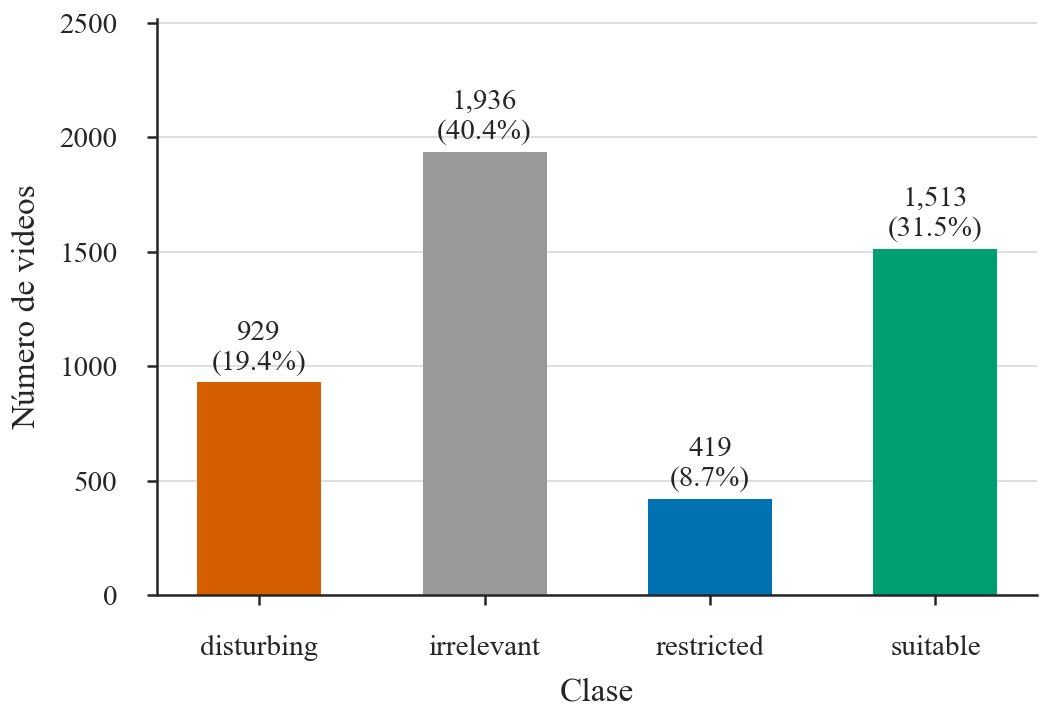
\includegraphics[width=\columnwidth]{images/distrib_clases_groundtruth.png}
\caption{Distribución de clases en el ground truth (número de videos y porcentaje).}
\label{fig:clases}
\end{figure}

La clase mayoritaria es \textit{irrelevant} (40.4\%), seguida de \textit{suitable} (31.5\%). Las clases de interés para la detección (\textit{disturbing} y \textit{restricted}) representan el 28.1\% del dataset, y \textit{restricted} es 4.6 veces más pequeña que la clase mayoritaria. Este nivel de desbalance deberá considerarse en el entrenamiento del modelo.

% ----- [ADRIÁN] -----
\subsection{Valores faltantes y calidad de los datos}\label{sec:faltantes}
La Fig.~\ref{fig:faltantes} muestra los valores faltantes por variable. \texttt{tags} es la más afectada (883 videos, 18.4\%), seguida de \texttt{description} (506, 10.5\%), \texttt{comment\_count} (228, 4.8\%), y \texttt{like\_count} y \texttt{dislike\_count} (128 cada una, 2.7\%). \texttt{view\_count} tiene 3 valores faltantes, y \texttt{duration\_seconds} y \texttt{definition} tienen 1 cada una. \texttt{title} y \texttt{category\_id} no presentan valores faltantes. La columna \texttt{prediction} está vacía en todo el ground truth (Sección~\ref{sec:leak}). Los conteos de datos válidos por variable numérica se muestran en la Tabla~\ref{tab:desc}. Además, 11 videos tienen 0 vistas y 10 tienen duración igual a 0, lo que exigirá tratar la división por cero al construir razones de interacción en el preprocesamiento. No se encontraron videos duplicados (mismo \texttt{video\_id}): los 4,797 registros son únicos.

\begin{figure}[!t]
\centering
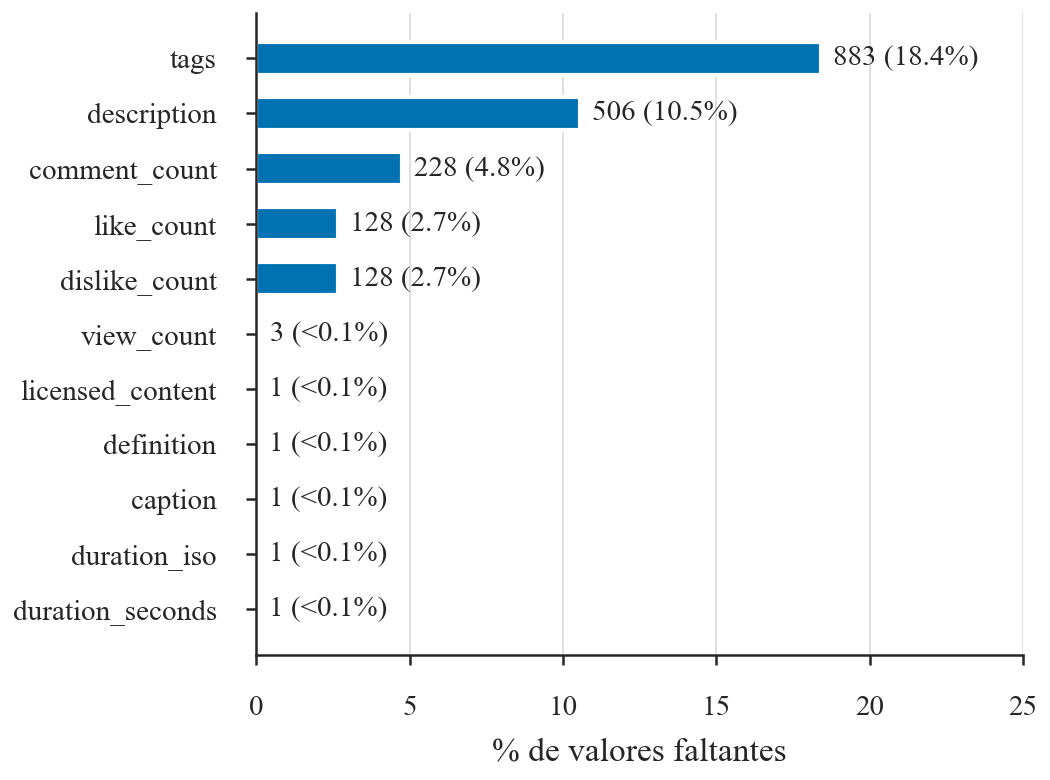
\includegraphics[width=\columnwidth]{images/valores_faltantes_groundtruth.png}
\caption{Porcentaje de valores faltantes por variable en el ground truth, con el número de videos entre paréntesis (se omite \texttt{prediction}, vacía en el 100\% de los registros).}
\label{fig:faltantes}
\end{figure}

% ----- [MAFER] -----
\subsection{Estadísticas descriptivas}
La Tabla~\ref{tab:desc} resume las variables numéricas del ground truth. Las métricas de interacción presentan alta variabilidad: por ejemplo, la media de \texttt{view\_count} (6,142,716.96) es muy superior a su mediana (90,093.5). La duración promedio es de 752.06 s (12.5 min), mientras que la mediana es de 345.5 s (5.8 min). Los máximos muestran outliers significativos, sobre todo en visualizaciones y duración (Sección~\ref{sec:outliers}).

\begin{table*}[!t]
\caption{Estadísticas descriptivas de las variables numéricas del ground truth}
\begin{center}
\footnotesize
\begin{tabular}{|l|r|r|r|r|r|r|r|r|}
\hline
\textbf{Variable} & \textbf{Válidos} & \textbf{Media} & \textbf{Desv. est.} & \textbf{Mín.} & \textbf{P25} & \textbf{Mediana} & \textbf{P75} & \textbf{Máx.} \\
\hline
\texttt{view\_count} & 4,794 & 6,142,716.96 & 43,836,538.05 & 0 & 1,140 & 90,093.50 & 1,775,452.75 & 1,664,660,083 \\
\hline
\texttt{like\_count} & 4,669 & 26,878.13 & 155,478.81 & 0 & 10 & 502.00 & 10,122 & 4,392,637 \\
\hline
\texttt{dislike\_count} & 4,669 & 3,718.92 & 25,425.08 & 0 & 1 & 53.00 & 1,097 & 1,071,513 \\
\hline
\texttt{comment\_count} & 4,569 & 2,378.41 & 12,849.85 & 0 & 1 & 49.00 & 763 & 323,267 \\
\hline
\texttt{duration\_seconds} & 4,796 & 752.06 & 1,986.99 & 0 & 167 & 345.50 & 706.25 & 39,433 \\
\hline
\end{tabular}
\label{tab:desc}
\end{center}
\end{table*}

% ----- [MAFER] -----
\subsection{Análisis por clase}
La Tabla~\ref{tab:clase} compara las variables numéricas y de título entre clases. \textit{Suitable} presenta la mayor media de vistas (10,761,959.60), mientras que \textit{restricted} presenta la mayor mediana de vistas y la mayor media de comentarios. Las medias están fuertemente afectadas por outliers, por lo que las medianas ofrecen una comparación más robusta (Fig.~\ref{fig:eng_vl}). Por ello, no es correcto atribuir el mayor nivel de interacción a la clase \textit{disturbing}.

\begin{table*}[!t]
\caption{Estadísticas por clase}
\begin{center}
\footnotesize
\begin{tabular}{|l|r|r|r|r|}
\hline
\textbf{Medida} & \textbf{Disturbing} & \textbf{Irrelevant} & \textbf{Restricted} & \textbf{Suitable} \\
\hline
Vistas (mediana) & 39,144 & 10,436 & 1,348,394 & 407,330 \\
\hline
Likes (mediana) & 202 & 87 & 5,130 & 1,342 \\
\hline
Comentarios (mediana) & 27 & 14 & 531 & 69.5 \\
\hline
Duración, s (mediana) & 359 & 264 & 350 & 443.5 \\
\hline
Título, caracteres (media) & 58.98 & 46.80 & 44.79 & 61.88 \\
\hline
Título, palabras (media) & 10.04 & 8.12 & 7.79 & 10.91 \\
\hline
\end{tabular}
\label{tab:clase}
\end{center}
\end{table*}

\begin{figure}[!t]
\centering
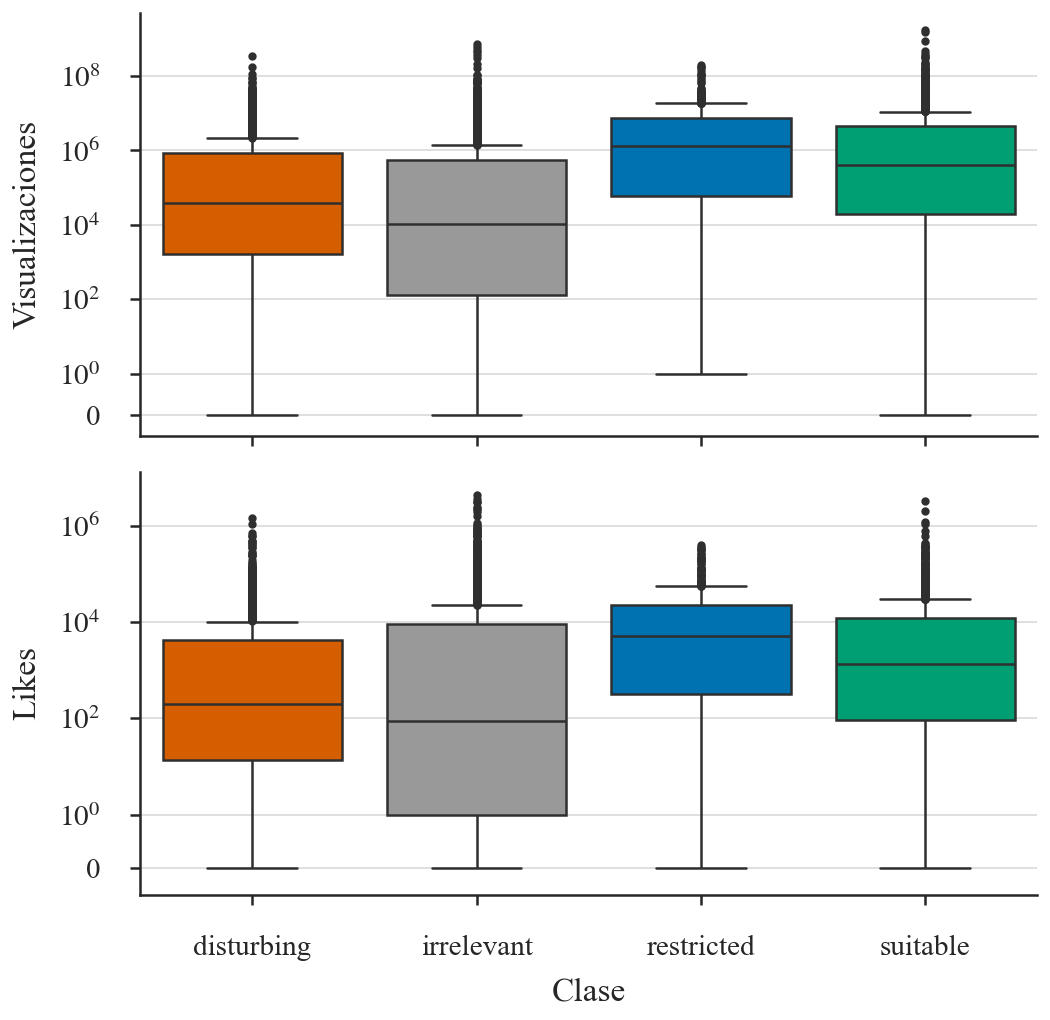
\includegraphics[width=\columnwidth]{images/distrib_engagement_vistas_likes_groundtruth.png}
\caption{Vistas y likes por clase (diagramas de caja en escala logarítmica simétrica, lineal cerca de cero para representar los videos con valor 0).}
\label{fig:eng_vl}
\end{figure}

\textit{Duración.} \textit{Suitable} tiene la mayor duración media (872.00 s) y mediana (443.5 s). Las medianas se sitúan entre 264 y 443.5 s (4.4 a 7.4 min), y la variabilidad es especialmente alta en \textit{irrelevant} y \textit{suitable} por la presencia de videos muy largos (Fig.~\ref{fig:dur_box}).

\begin{figure}[!t]
\centering
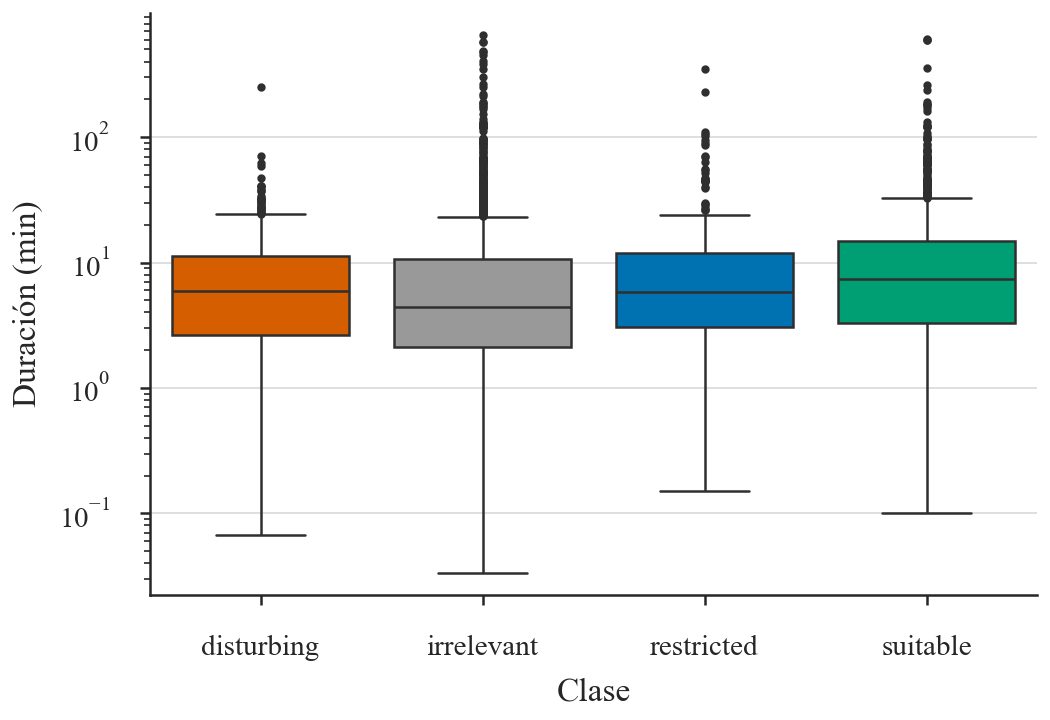
\includegraphics[width=\columnwidth]{images/distrib_duracion_box_groundtruth.png}
\caption{Duración por clase (diagrama de caja, escala logarítmica). Se excluyen los 10 videos con duración 0.}
\label{fig:dur_box}
\end{figure}

\textit{Categorías y definición.} El dataset abarca 17 categorías de YouTube (Fig.~\ref{fig:categ}; los nombres provienen de la YouTube Data API~\cite{ytapi}). Las tres más frecuentes son \textit{Entertainment}, \textit{People \& Blogs} y \textit{Film \& Animation}, y algunas categorías predominan en ciertas clases. Respecto a la calidad, 3,748 videos (78.1\%) están en HD y 1,048 (21.8\%) en SD. La asociación entre la definición y la clase es estadísticamente significativa ($\chi^2=23.30$, $p=3.5\times10^{-5}$), pero muy débil ($V$ de Cramér $=0.07$), por lo que la calidad del video no parece estar directamente relacionada con la clasificación de contenido.

\begin{figure}[!t]
\centering
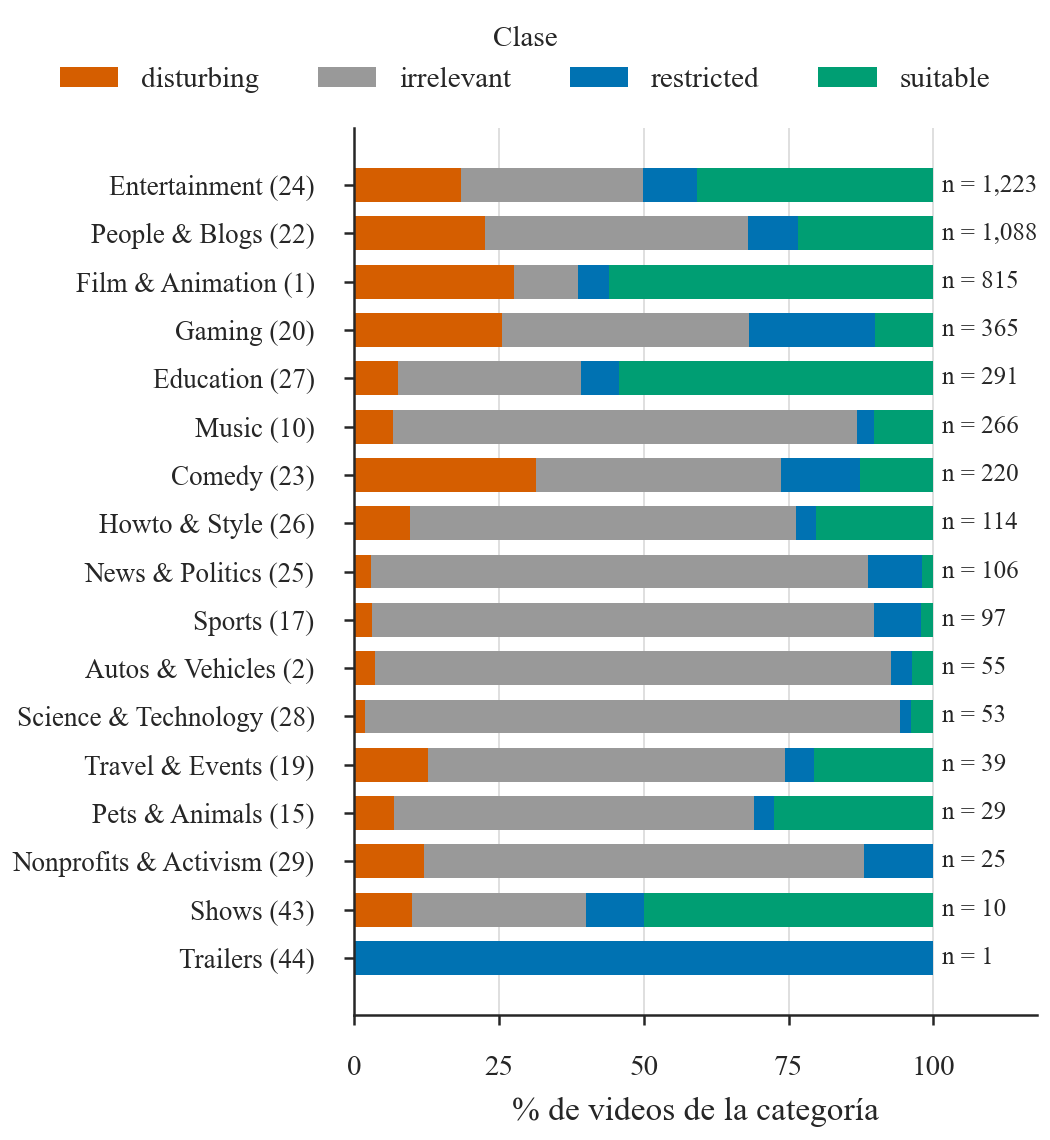
\includegraphics[width=\columnwidth]{images/distrib_categ_etiqueta_groundtruth.png}
\caption{Composición por clase de cada categoría de YouTube, ordenadas por número de videos ($n$; entre paréntesis, el ID de categoría). Los porcentajes de las categorías con pocos videos son poco fiables.}
\label{fig:categ}
\end{figure}

\textit{Títulos.} Los títulos tienen en promedio 53.74 caracteres y 9.34 palabras. Los títulos de \textit{suitable} tienen la mayor longitud media (61.88 caracteres) y cantidad media de palabras (10.91), seguidos por los de \textit{disturbing}, mientras que \textit{restricted} presenta los títulos más cortos en promedio (Tabla~\ref{tab:clase}). La longitud del título podría ser una característica discriminante.

\textit{Etiquetas (tags).} 3,914 videos tienen tags y 883 (18.4\%) no tienen. Esos registros contienen 3,705 listas de tags distintas; al separar cada lista por \texttt{|} (eliminando espacios y cadenas vacías) se obtienen 40,096 tags individuales únicos y 73,640 asignaciones en total (18.8 tags por video en promedio). Al normalizar a minúsculas se consolidan 36,750 tags únicos, y la Tabla~\ref{tab:tags} usa esta versión, contando cada tag una sola vez por video. Al cruzar los tags individuales más frecuentes con la clase se observan asociaciones marcadas: el 74.6\% de los videos con el tag \textit{spiderman} son \textit{disturbing}, frente al 19.4\% en todo el ground truth, mientras que el 80.1\% de los videos con \textit{for kids} son \textit{suitable}, frente al 31.5\%. Los tags \textit{spiderman}, \textit{superhero}, \textit{elsa} y \textit{frozen} se distribuyen en 181, 133, 171 y 169 canales distintos, respectivamente, y el canal con más videos de cada uno aporta menos del 4\% del total, por lo que su asociación con \textit{disturbing} no depende de un solo canal. En cambio, para \textit{kids} (412 videos en 270 canales) y \textit{children} (215 videos en 129 canales), un único canal, el mismo que aparece con clases mixtas en la Sección~\ref{sec:leak}, aporta el 7.3\% y el 14.4\% de los videos, respectivamente. Estas asociaciones son descriptivas y su capacidad predictiva deberá confirmarse en el modelado.

\begin{table}[!t]
\caption{Tags individuales frecuentes (en minúsculas): \% de videos por clase}
\begin{center}
\footnotesize
\setlength{\tabcolsep}{3pt}
\begin{tabular}{|l|r|r|r|r|r|}
\hline
\textbf{Tag} & \textbf{Videos} & \textbf{Dist.} & \textbf{Irrel.} & \textbf{Restr.} & \textbf{Suit.} \\
\hline
spiderman & 209 & 74.6 & 4.3 & 1.9 & 19.1 \\
\hline
superhero & 156 & 74.4 & 6.4 & 0.6 & 18.6 \\
\hline
elsa & 200 & 60.0 & 6.0 & 3.0 & 31.0 \\
\hline
frozen & 194 & 57.7 & 5.7 & 2.6 & 34.0 \\
\hline
funny & 400 & 39.5 & 19.0 & 6.5 & 35.0 \\
\hline
kids & 412 & 31.1 & 4.6 & 1.2 & 63.1 \\
\hline
children & 215 & 20.9 & 7.9 & 0.0 & 71.2 \\
\hline
cartoon & 299 & 24.7 & 2.7 & 0.3 & 72.2 \\
\hline
for kids & 136 & 12.5 & 4.4 & 2.9 & 80.1 \\
\hline
\textit{Ground truth} & 4,797 & 19.4 & 40.4 & 8.7 & 31.5 \\
\hline
\end{tabular}
\label{tab:tags}
\end{center}
\end{table}

% ----- [ADRIÁN] -----
\subsection{Detección de outliers}\label{sec:outliers}
Se aplicó el método del rango intercuartílico (IQR) sobre las cinco variables numéricas, tanto en su escala original como sobre una transformación logarítmica $\log(1+x)$ (Tabla~\ref{tab:out}, Fig.~\ref{fig:box}). Esta segunda versión es necesaria porque, dada la fuerte asimetría de las métricas de interacción, el IQR en escala original marca como outlier a una fracción muy grande de las observaciones (entre 15.6\% y 16.9\%), lo cual no es informativo.

En escala logarítmica, el número de outliers en las cuatro variables de interacción desciende a 0, lo que muestra que las observaciones siguen una distribución log-normal coherente y que no constituyen errores ni datos anómalos. Únicamente \texttt{duration\_seconds} retiene 173 outliers (3.61\%), correspondientes a videos notablemente cortos o largos. Al cruzar los valores extremos de vistas ($>$4.4M) y likes ($>$25.3K) con la clase, se observa que están repartidos entre todas las clases (en vistas: 379 \textit{suitable}, 175 \textit{irrelevant}, 132 \textit{restricted} y 116 \textit{disturbing}). Por ello, corresponden a contenido popular legítimo dentro de cada categoría y no deben descartarse, sino transformarse mediante $\log(1+x)$ en la etapa 2.

\begin{table}[!t]
\caption{Outliers detectados por el método IQR}
\begin{center}
\footnotesize
\begin{tabular}{|l|r|r|r|r|}
\hline
 & \multicolumn{2}{c|}{\textbf{Escala original}} & \multicolumn{2}{c|}{\textbf{Escala log}} \\
\cline{2-5}
\textbf{Variable} & \textbf{N.°} & \textbf{\%} & \textbf{N.°} & \textbf{\%} \\
\hline
\texttt{view\_count} & 802 & 16.73 & 0 & 0.00 \\
\hline
\texttt{like\_count} & 730 & 15.64 & 0 & 0.00 \\
\hline
\texttt{dislike\_count} & 791 & 16.94 & 0 & 0.00 \\
\hline
\texttt{comment\_count} & 721 & 15.78 & 0 & 0.00 \\
\hline
\texttt{duration\_seconds} & 385 & 8.03 & 173 & 3.61 \\
\hline
\end{tabular}
\label{tab:out}
\end{center}
\end{table}

\begin{figure*}[!t]
\centering
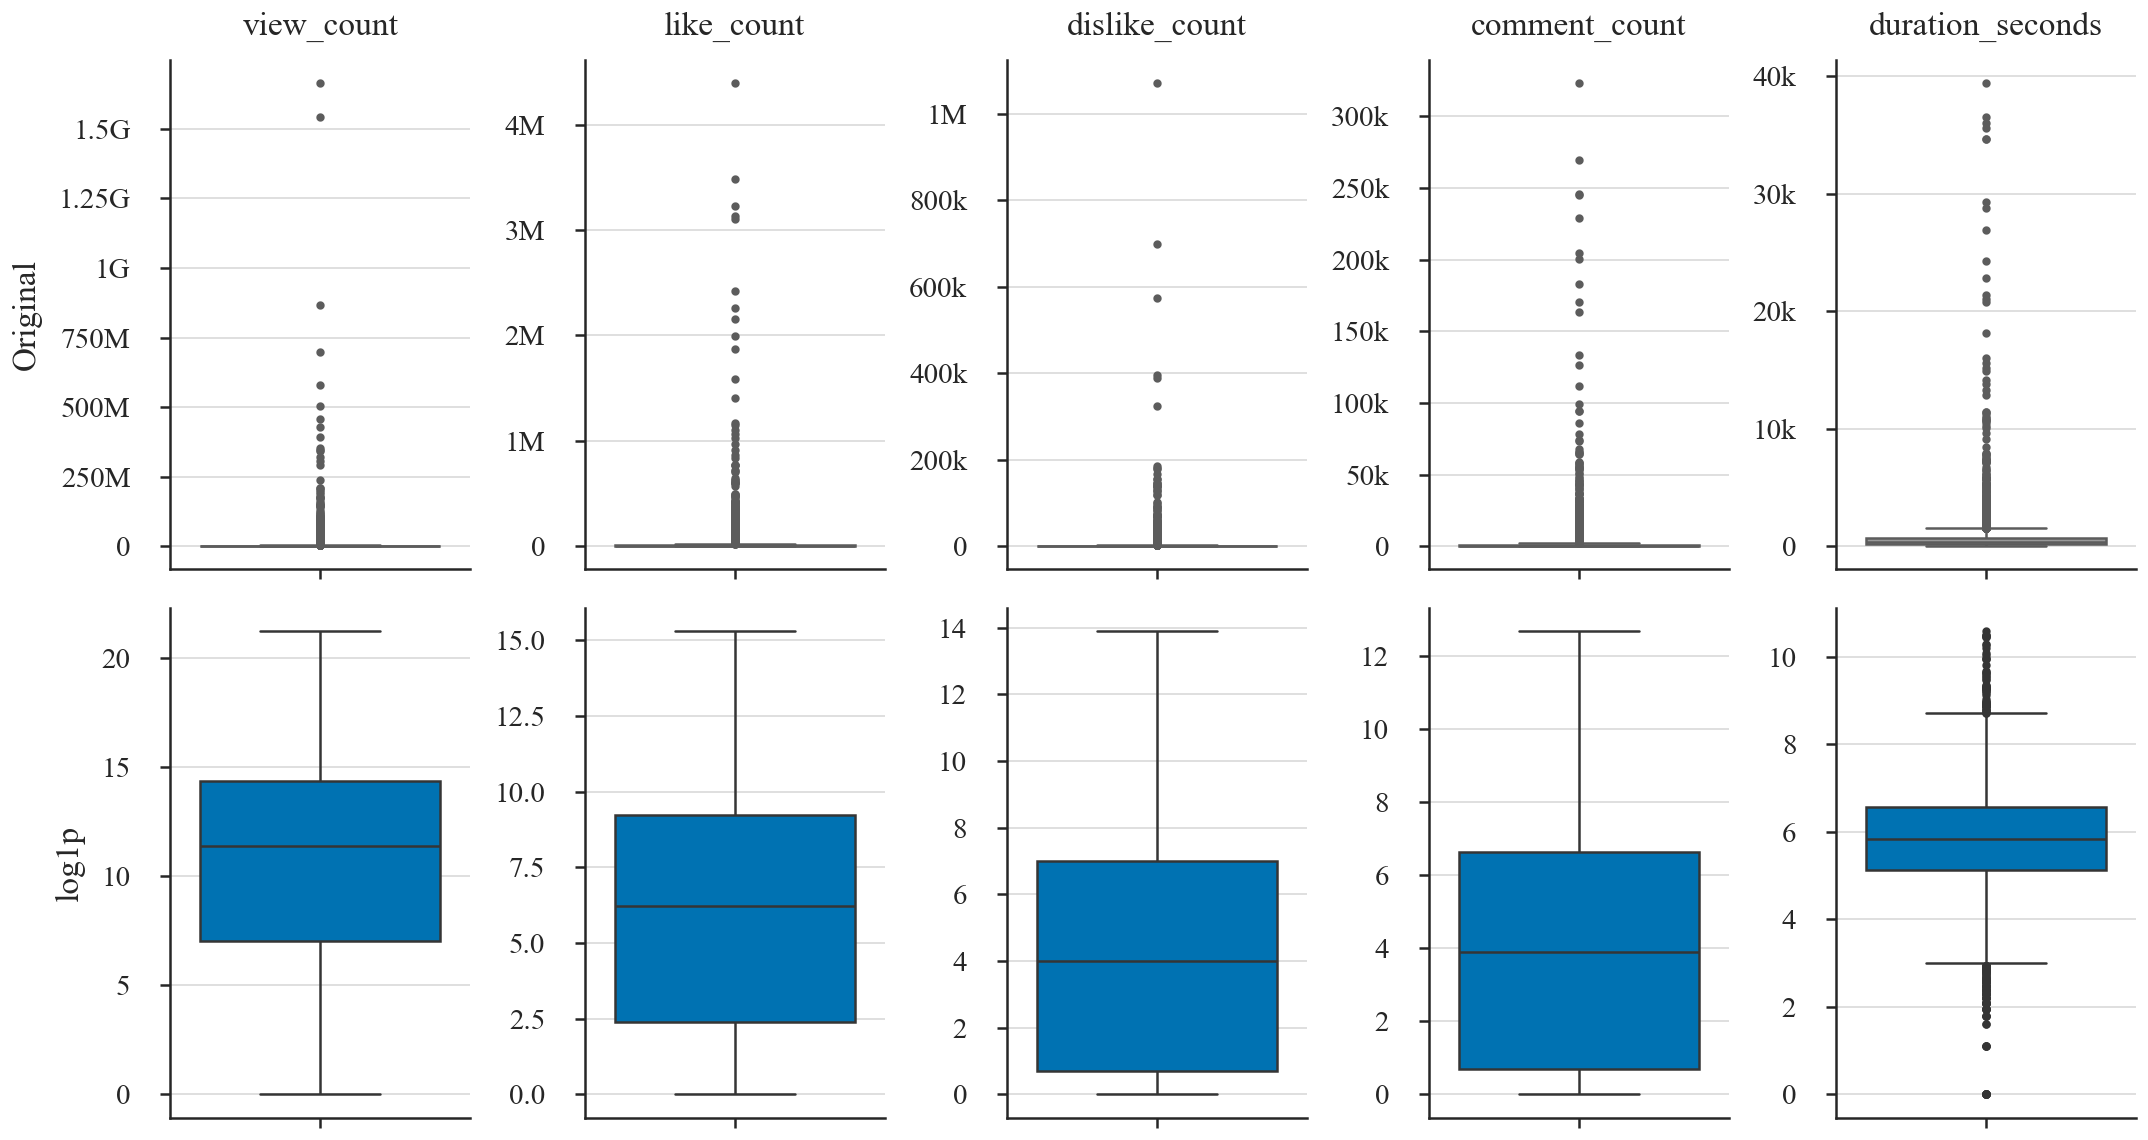
\includegraphics[width=\textwidth]{images/outliers_boxplots_groundtruth.png}
\caption{Diagramas de caja de las variables numéricas en escala original (arriba) y logarítmica $\log(1+x)$ (abajo).}
\label{fig:box}
\end{figure*}

% ----- [ADRIÁN] -----
\subsection{Relaciones entre variables}\label{sec:corr}
Se analizó la correlación entre las variables numéricas (Pearson en escala original y logarítmica, y Spearman) para identificar redundancia y posibles problemas de multicolinealidad (la Fig.~\ref{fig:corr_spearman} muestra la matriz de Spearman). Las métricas de interacción presentan una correlación excepcionalmente alta entre sí: \texttt{view\_count} y \texttt{dislike\_count} (Spearman 0.966, Pearson log 0.940), \texttt{view\_count} y \texttt{like\_count} (Spearman 0.956, Pearson log 0.955), y \texttt{like\_count} y \texttt{comment\_count} (Spearman 0.948, Pearson log 0.947). Esta colinealidad casi unitaria desaconseja emplear los cuatro conteos como variables directas simultáneas; en su lugar, se deben formular razones normalizadas (likes/vistas, comentarios/vistas). Por su parte, \texttt{duration\_seconds} mantiene correlaciones bajas con las variables de interacción (Pearson log entre 0.228 y 0.241, Spearman entre 0.217 y 0.225), por lo que provee una señal complementaria e independiente.

\begin{figure}[!t]
\centering
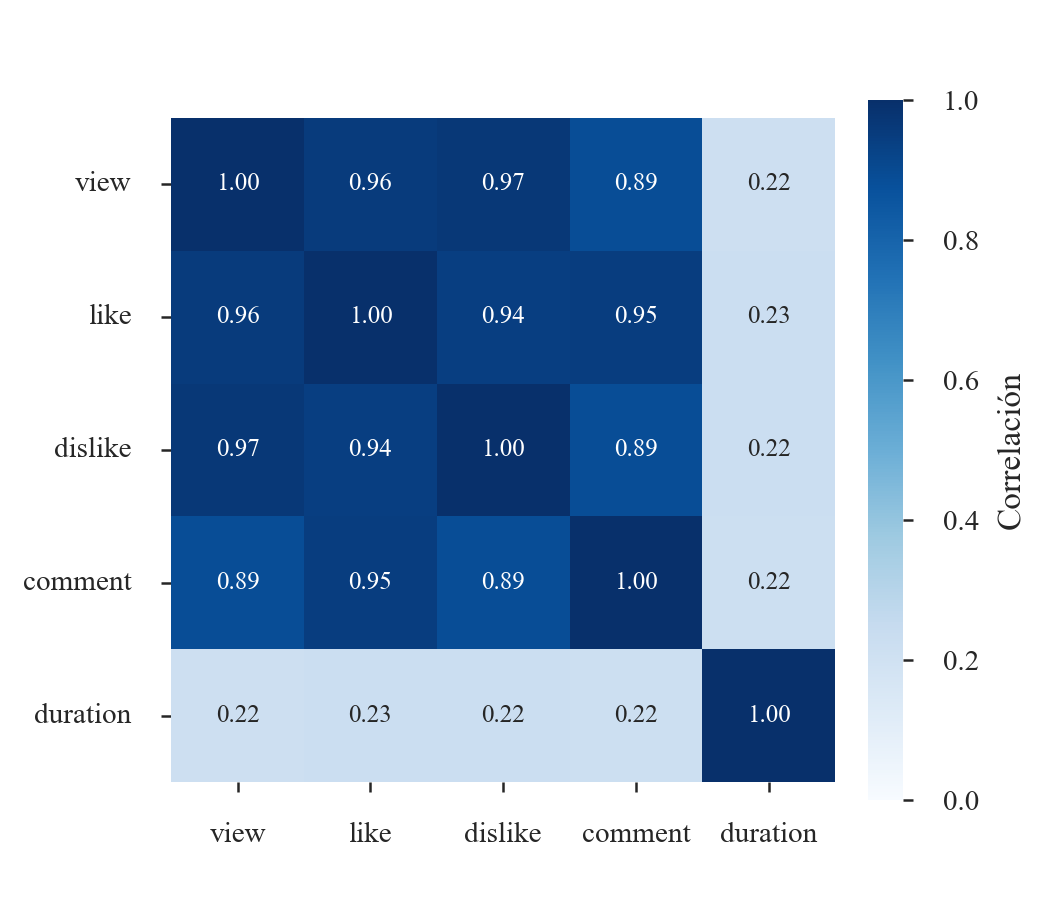
\includegraphics[width=\columnwidth]{images/correlacion_spearman_groundtruth.png}
\caption{Correlación de Spearman entre las variables numéricas (los valores de Pearson en escala $\log(1+x)$ se reportan en el texto).}
\label{fig:corr_spearman}
\end{figure}

Adicionalmente, se aplicó la prueba de Kruskal-Wallis para evaluar si la distribución de cada variable numérica difiere de forma estadísticamente significativa entre las cuatro clases (Tabla~\ref{tab:kw}). Las cinco variables resultaron significativas ($p<0.05$; de hecho, todas con $p<10^{-27}$). No obstante, dado el tamaño muestral (${\sim}$4,800 observaciones), diferencias distributivas pequeñas pueden alcanzar significancia con facilidad; por ello, este resultado funciona como un filtro preliminar positivo (ninguna variable se descarta a priori), y su capacidad predictiva deberá confirmarse en la etapa 2 mediante métricas de importancia de características con los modelos entrenados.

\begin{table}[!t]
\caption{Prueba de Kruskal-Wallis: variable numérica vs. clase}
\begin{center}
\footnotesize
\begin{tabular}{|l|r|r|}
\hline
\textbf{Variable} & \textbf{Estadístico $H$} & \textbf{$p$-valor} \\
\hline
\texttt{view\_count} & 523.87 & $3.20\times10^{-113}$ \\
\hline
\texttt{like\_count} & 232.61 & $3.76\times10^{-50}$ \\
\hline
\texttt{dislike\_count} & 399.39 & $3.00\times10^{-86}$ \\
\hline
\texttt{comment\_count} & 150.65 & $1.91\times10^{-32}$ \\
\hline
\texttt{duration\_seconds} & 129.94 & $5.57\times10^{-28}$ \\
\hline
\end{tabular}
\label{tab:kw}
\end{center}
\end{table}

% ----- [MAFER] -----
\subsection{Conjuntos adicionales}\label{sec:adic}
Se analizaron las primeras 1,000 líneas del primer archivo de cada conjunto adicional. No son muestras aleatorias y en ellas predominan videos que también están en el ground truth (780 en \texttt{elsagate\_related}, 70 en \texttt{other\_child\_related}, 34 en \texttt{random\_videos} y 490 en \texttt{popular\_videos}), por lo que los porcentajes de videos predichos como inapropiados no representan la prevalencia en los conjuntos completos. Como muestra la Tabla~\ref{tab:add}, casi todos los videos predichos como inapropiados pertenecen al ground truth: en \texttt{elsagate\_related}, 472 de los 780 videos del ground truth (60.5\%) fueron predichos como inapropiados, frente a 1 de los 220 restantes (0.5\%); en los otros tres conjuntos, ningún video fuera del ground truth fue predicho como inapropiado. Fuera del ground truth solo existe la predicción automática del clasificador, sin etiquetas humanas.

Para no depender de estas primeras líneas, se revisó también el corpus consolidado completo (844,702 videos únicos), en el que cada video del ground truth aparece una sola vez y queda separado de los conjuntos adicionales. Fuera del ground truth, el clasificador original predijo como inapropiados 1,260 de 230,873 videos de \texttt{elsagate\_related} (0.55\%), 586 de 137,043 de \texttt{other\_child\_related} (0.43\%), 3,388 de 462,382 de \texttt{random\_videos} (0.73\%) y ninguno de los 9,607 de \texttt{popular\_videos}. Por tanto, la ausencia de videos inapropiados fuera del ground truth en la Tabla~\ref{tab:add} es un efecto de la muestra analizada y no se mantiene en los conjuntos completos. Como el consolidado asigna un único conjunto de origen a cada video, un video presente en varios conjuntos se cuenta solo en uno.

\begin{table}[!t]
\caption{Videos predichos como inapropiados en las primeras 1,000 líneas de cada conjunto adicional$^{\mathrm{a}}$}
\begin{center}
\footnotesize
\setlength{\tabcolsep}{3pt}
\begin{tabular}{|l|r|r|r|r|}
\hline
 & \multicolumn{2}{c|}{\textbf{Videos}} & \multicolumn{2}{c|}{\textbf{Inapropiados}} \\
\cline{2-5}
\textbf{Conjunto} & \textbf{En GT} & \textbf{Fuera} & \textbf{En GT} & \textbf{Fuera} \\
\hline
Elsagate & 780 & 220 & 472 (60.5\%) & 1 (0.5\%) \\
\hline
Other child & 70 & 930 & 15 (21.4\%) & 0 (0.0\%) \\
\hline
Random & 34 & 966 & 3 (8.8\%) & 0 (0.0\%) \\
\hline
Popular & 490 & 510 & 27 (5.5\%) & 0 (0.0\%) \\
\hline
\multicolumn{5}{l}{\scriptsize $^{\mathrm{a}}$GT: ground truth. Predicción automática del clasificador.}
\end{tabular}
\label{tab:add}
\end{center}
\end{table}

% ----- [ADRIÁN] -----
\subsection{Posible fuga de datos (data leakage)}\label{sec:leak}
Se revisaron cuatro fuentes potenciales de fuga de datos relevantes para el diseño experimental de la etapa 2:
\begin{enumerate}
\item \textbf{Columnas que codifican la etiqueta o la predicción original.} \texttt{prediction} e \texttt{is\_ground\_truth} son generadas por el clasificador automático de los autores del dataset y por el proceso de anotación, respectivamente. No son información disponible de forma independiente para un video nuevo, por lo que no deben usarse como características. En el ground truth, \texttt{prediction} contiene 100\% de valores nulos (4,797 registros) e \texttt{is\_ground\_truth} toma el valor constante 1.
\item \textbf{Duplicados dentro del ground truth.} Se constató que existen 0 videos duplicados (mismo \texttt{video\_id}); los 4,797 registros son videos únicos. De existir duplicados, un mismo video repetido en entrenamiento y validación inflaría artificialmente el desempeño.
\item \textbf{Solapamiento entre ground truth y conjuntos adicionales.} Como el ground truth se usa para entrenar y los conjuntos adicionales para comprobación de consistencia, un video presente en ambos dejaría de ser una prueba genuina de generalización. La Tabla~\ref{tab:add} muestra los videos en común (sobre las 1,000 líneas analizadas): 780 (78.0\%) en \texttt{elsagate\_related}, 70 (7.0\%) en \texttt{other\_child\_related}, 34 (3.4\%) en \texttt{random\_videos} y 490 (49.0\%) en \texttt{popular\_videos}. Estos videos deberán excluirse de la comprobación.
\item \textbf{Concentración de videos por canal.} El ground truth contiene 3,818 canales únicos (por \texttt{channel\_id}), de los cuales 418 tienen más de un video (máximo de 33 videos para un canal). Entre los 13 canales con 12 o más videos (seis empatan con exactamente 12), 11 concentran el 100\% en \textit{suitable}, uno tiene el 91.7\% en \textit{suitable} (11 \textit{suitable} y 1 \textit{disturbing}) y solo uno (33 videos) presenta mezcla de clases (20 \textit{disturbing} y 13 \textit{suitable}). Esto implica riesgo de que el modelo memorice características propias del canal, y de fuga de datos si videos del mismo canal quedan repartidos entre entrenamiento y validación o prueba. Se recomienda una partición agrupada por canal (por ejemplo, \texttt{StratifiedGroupKFold}, tanto para el conjunto de prueba como para la validación cruzada) además de la estratificación por clase.
\end{enumerate}

% ----- [ADRIÁN] -----
\subsection{Limitaciones}
Los conjuntos adicionales se analizaron solo con las primeras 1,000 líneas de un archivo, que no son muestras aleatorias y no representan la distribución de los conjuntos completos. Los datos corresponden a un periodo específico (2018) y YouTube ha cambiado significativamente desde entonces, por lo que los patrones pueden haber evolucionado. Además, las etiquetas manuales pueden contener sesgos subjetivos de los anotadores humanos.

% =====================================================================
% PREPROCESAMIENTO E INGENIERÍA DE CARACTERÍSTICAS  [MARIELA]
% =====================================================================
\section{Preprocesamiento e Ingeniería de Características}\label{sec:prep}
El preprocesamiento se implementó en \texttt{data\_processing/preprocessing.py} y genera \texttt{dataset\_features\_v1.csv}, con los 4,797 videos del ground truth, 16 características, la etiqueta y tres columnas de metadatos (\texttt{video\_id}, \texttt{channel\_id} y \texttt{split}) que no se usan como características. Para evitar fuga de datos, todos los valores que se aprenden de los datos (medianas, modas y vocabularios) se ajustan solo con el conjunto de entrenamiento.

\subsection{Partición previa}
Antes de transformar los datos se reservó el conjunto de prueba con \texttt{StratifiedGroupKFold} (5 particiones, semilla 42), estratificando por clase y agrupando por \texttt{channel\_id}, y se tomó la primera partición como prueba: 3,842 videos de entrenamiento y 955 de prueba (19.9\%), sin canales en común (Sección~\ref{sec:leak}). Así, las estadísticas de imputación no incorporan información del conjunto de prueba.

\subsection{Transformaciones aplicadas}
\begin{itemize}
\item \textbf{Valores faltantes numéricos:} \texttt{like\_count}, \texttt{dislike\_count} (128), \texttt{comment\_count} (228), \texttt{view\_count} (3) y \texttt{duration\_seconds} (1) se imputan con la mediana de entrenamiento, robusta frente a la fuerte asimetría observada (Tabla~\ref{tab:desc}).
\item \textbf{Valores faltantes categóricos:} \texttt{definition}, \texttt{caption} y \texttt{licensed\_content} (1 faltante cada una) se imputan con la moda de entrenamiento.
\item \textbf{Texto faltante:} la ausencia de descripción (506) o de tags (883) se representa como texto vacío, sin inventar contenido. Los tags se normalizan a minúsculas y se separan por \texttt{|}, como en el análisis de la Sección~\ref{sec:target}.
\item \textbf{Transformación logarítmica:} los cuatro conteos de interacción se transforman con $\log(1+x)$, que elimina los outliers detectados por el IQR (Tabla~\ref{tab:out}) sin descartar videos.
\item \textbf{Codificación y escalamiento:} \texttt{category\_id}, \texttt{definition}, \texttt{caption} y \texttt{licensed\_content} se codifican con one-hot (las categorías con menos de 5 videos se agrupan), y las variables numéricas se estandarizan.
\end{itemize}

\subsection{Características derivadas}
\begin{itemize}
\item \textbf{Razones de interacción:} likes/vistas y comentarios/vistas, que sustituyen el uso conjunto de conteos casi colineales (Sección~\ref{sec:corr}). Si faltan los conteos o las vistas son 0 (11 videos), la razón queda indefinida y se imputa con la mediana de entrenamiento.
\item \textbf{Longitud del título:} número de caracteres y de palabras. Sus medias reproducen las de la Tabla~\ref{tab:clase} (alrededor de 60 caracteres en \textit{suitable} y \textit{disturbing} frente a 45 en \textit{irrelevant} y \textit{restricted}).
\item \textbf{Representación del texto:} TF-IDF con frecuencia sublineal y sin acentos sobre el título y la descripción (unigramas y bigramas) y sobre los tags, tratando cada tag completo como un token (por ejemplo, \textit{for kids}). Ajustado con el conjunto de entrenamiento genera 4,985 columnas para el título, 27,344 para la descripción y 5,927 para los tags. Para los modelos de árboles, este bloque puede reducirse con \texttt{TruncatedSVD}.
\end{itemize}
El texto se vectoriza dentro de un \texttt{Pipeline} de scikit-learn, de modo que en la validación cruzada el vocabulario y los pesos IDF se ajustan solo con las particiones de entrenamiento. La Tabla~\ref{tab:terms} muestra los tags con mayor asociación a cada clase en entrenamiento (prueba $\chi^2$, una clase contra el resto). Coinciden con los hallazgos del EDA, pero algunos términos corresponden a series o canales concretos (por ejemplo, \textit{tom and jerry} o \textit{prankzone tv}), lo que confirma la necesidad de validar agrupando por canal.

\begin{table}[!t]
\caption{Tags más asociados a cada clase en entrenamiento ($\chi^2$)}
\begin{center}
\footnotesize
\begin{tabular}{|l|p{6.2cm}|}
\hline
\textbf{Clase} & \textbf{Tags} \\
\hline
Disturbing & spiderman, superhero, mlg, spidey, spider-man, joker, elsa \\
\hline
Irrelevant & srbija, pop, 2016, rap, comedian, sports \\
\hline
Restricted & sexy, sex, prankzone tv, playstation 4, hot, hypnosis \\
\hline
Suitable & tom and jerry, cartoon, kids, animation, animated cartoon \\
\hline
\end{tabular}
\label{tab:terms}
\end{center}
\end{table}

\subsection{Variables excluidas}
No se usan como características \texttt{prediction} e \texttt{is\_ground\_truth} (codifican el proceso de clasificación o de anotación), \texttt{source\_dataset} (constante), \texttt{favorite\_count} (siempre 0), \texttt{published\_at} y \texttt{duration\_iso} (redundante con \texttt{duration\_seconds}), ni los identificadores \texttt{video\_id}, \texttt{channel\_id} y \texttt{channel\_title}, para que el modelo no memorice canales (Sección~\ref{sec:leak}); \texttt{channel\_id} se conserva solo para agrupar la partición. Las mismas transformaciones, con los valores de imputación de entrenamiento, se aplican a los conjuntos adicionales.

% =====================================================================
% SIGUIENTES PASOS  [MAFER]
% =====================================================================
\section{Propuesta de Siguientes Pasos}\label{sec:next}
\begin{enumerate}
\item \textbf{Feature Engineering:} aplicar $\log(1+x)$ a las métricas de interacción, crear razones (likes/vistas, comentarios/vistas) e implementar técnicas de NLP para analizar títulos, descripciones y tags (normalizar tags a minúsculas, TF-IDF o embeddings). Se excluyen \texttt{prediction}, \texttt{is\_ground\_truth}, \texttt{video\_id}, \texttt{channel\_id} y \texttt{channel\_title} como características.
\item \textbf{Modelado baseline:} definir un baseline de referencia (clasificador que predice siempre la clase mayoritaria) y comparar modelos que permitan aislar el aporte de cada tipo de información: por ejemplo, regresión logística con TF-IDF para el texto, un modelo de árboles (LightGBM o Random Forest) para los metadatos y un modelo combinado de ambos. La selección final se justificará en la segunda etapa según los resultados. El desbalance de clases se abordará con class weights o SMOTE.
\item \textbf{Modelos avanzados:} explorar embeddings preentrenados o transformers para texto solo si el texto resulta ser la señal más fuerte en la etapa anterior. El uso de thumbnails (CNN) queda como extensión.
\item \textbf{Validación:} reservar cerca del 20\% del ground truth como conjunto de prueba, estratificado por clase y agrupado por canal (Sección~\ref{sec:leak}), y aplicar validación cruzada con el mismo criterio sobre el resto. La evaluación se centrará en el F1 macro y por clase, en lugar de la exactitud, que se vería distorsionada por el desbalance de hasta 4.6 veces a favor de la clase mayoritaria, y se priorizará el recall en las clases críticas (\textit{restricted} y \textit{disturbing}). Las transformaciones (imputación, TF-IDF, SMOTE) se ajustarán solo con los datos de entrenamiento para prevenir fuga de datos.
\item \textbf{Pruebas en datasets adicionales:} aplicar el modelo final a los conjuntos adicionales, excluyendo los videos que ya están en el ground truth (Sección~\ref{sec:leak}). Como no tienen etiquetas humanas, sirven como comprobación de consistencia (proporción de videos predichos como inapropiados y acuerdo con \texttt{prediction}), no para medir la eficacia, que se mide en el conjunto de prueba reservado.
\end{enumerate}

% =====================================================================
% REFERENCIAS
% =====================================================================
\bibliographystyle{IEEEtran}
\nocite{urbina2026machinelearning}
\bibliography{references}

\end{document}